\documentclass{assignment}
\UsingEnglish
\ProjectInfos*{Intro to Communication System}{EE140}{Fall, 2020}{Assignment 6}{Due time : 10:15, Oct 30, 2020 (Friday)}{陈稼霖}{45875852}
\begin{document}
\begin{prob}[Noise in DSB-SC Receiver, 30pts]
    A DSB-SC modulated signal in transmitted over a noisy channel. The power spectral density of the noise is shown in Figure \ref{A-6-P-1}. The message bandwidth is $3$ kHz and the carrier frequency is $200$ kHz. Assuming that the average power of the modulated signal is $12$ watts, determine the input signal-to-noise ratio (predetection SNR), output signal-to-noise ratio (postdetection SNR) and the detection gain (output SNR / input SNR).
    \begin{figure}[h]
        \centering
        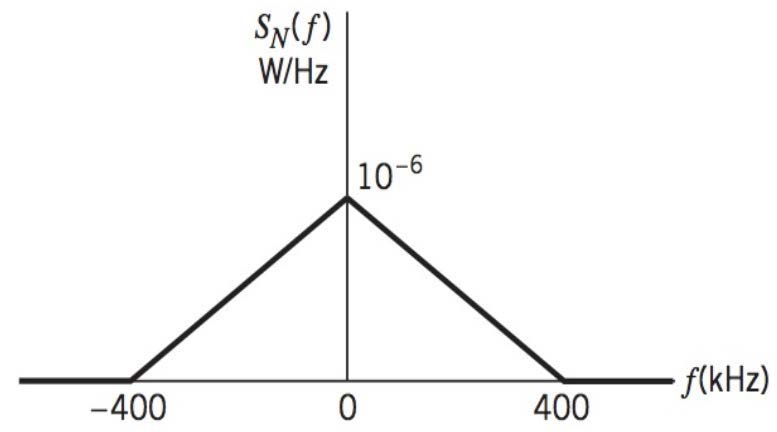
\includegraphics[width=.5\columnwidth]{A-6-P-1.jpg}
        \caption{}
        \label{A-6-P-1}
    \end{figure}
\end{prob}
\begin{sol}
    The received signal is the sum of the DSB-SC modulated signal and the noise:
    \begin{align}
        x_r(t)=x_c(t)+n(t)=A_cm(t)\cos(2\pi f_ct+\theta)+n(t)=A_c\cos(2\pi\cdot 200000t+\theta)+n(t).
    \end{align}
    After passing the bandpass filter, the received signal becomes
    \begin{align}
        \notag e_2(t)=&x_c(t)+n'(t)=A_c\cos(2\pi f_ct+\theta)+n_c\cos(2\pi f_ct+\theta)-n_s\sin(2\pi f_ct+\theta)\\
        =&A_c\cos(2\pi\cdot 200000t+\theta)+n_c\cos(2\pi\cdot 200000t)-n_s\sin(2\pi\cdot 200000t).
    \end{align}
    The average power of the modulated signal $x_c(t)$ is
    \begin{align}
        P_T=\frac{A_c^2}{2}\overline{m^2(t)}=12\mathrm{W}.
    \end{align}
    According to figure \ref{A-6-P-1}, the power spectral density of the noise is
    \begin{align}
        S_N(f)=10^{-6}\Lambda(400000f).
    \end{align}
    After passing the narrowband filter, the average power of the noise component is
    \begin{align}
        \notag P_{n'}=&\int_{-f_c-W}^{-f_c+W}S_N(f)\,\mathrm{d}f+\int_{f_c-W}^{f_c+W}S_N(f)\,\mathrm{d}f\\
        \notag=&2\int_{f_c-W}^{f_c+W}S_N(f)\,\mathrm{d}f\\
        \notag=&2\int_{200000-3000}^{200000+3000}10^{-6}\Lambda(400000f)\,\mathrm{d}f\\
        =&0.006(\mathrm{W}).
    \end{align}
    The input SNR is
    \begin{align}
        \text{SNR}_T=\frac{P_T}{P_{n'}}=\frac{12}{0.006}=2000.
    \end{align}
    After demodulation, the output is
    \begin{align}
        \notag y_D(t)=&\text{LP}[e_2(t)\cdot 2\cos(2\pi f_ct+\theta)]\\
        \notag=&\text{LP}\{A_cm(t)[1+\cos(4\pi f_ct+2\theta)]+n_c(t)[1+\cos(4\pi f_ct+2\theta)]-n_s(t)\sin(2\pi f_ct+2\theta)\}\\
        \notag=&A_cm(t)+n_c(t).
    \end{align}
    The average power of the demodulated signal component is
    \begin{align}
        A_c^2\overline{m^2(t)}=2P_T=24\mathrm{W}.
    \end{align}
    The average power of the noise component is
    \begin{align}
        P_{n_c}=P_{n'}=0.006\mathrm{W}.
    \end{align}
    The output SNR is
    \begin{align}
        \text{SNR}_D=\frac{2P_T}{P_{n_c}}=\frac{24}{0.006}=4000.
    \end{align}
    The detection gain is
    \begin{align}
        \frac{\text{SNR}_D}{\text{SNR}_T}=2.
    \end{align}
\end{sol}

\begin{prob}[Noise in SSB Receiver, 25pts]
    Derive the equation for $y_D(t)$ for an USB-SSB system assuming that the noise is expanded about the frequency $f_c+\frac{W}{2}$. Derive the output SNR (postdetection SNR), detection gain and the figure of merit. Determine and plot the power spectral density of the in-phase component $n_c(t)$ and the quadrature component $n_s(t)$ of the narrowband noise.
\end{prob}
\begin{sol}
    The USB-SSB modulated signal is
    \begin{align}
        x_c(t)=A_c[m(t)\cos(2\pi f_ct+\theta)-\hat{m}(t)\sin(2\pi f_ct+\theta)].
    \end{align}
    The received signal is
    \begin{align}
        x_r(t)=x_c(t)+w(t)=A_c[m(t)\cos(2\pi f_ct+\theta)-\hat{m}(t)\sin(2\pi f_ct+\theta)]+w(t).
    \end{align}
    After passing the band filter whose center frequency is $f_c+\frac{W}{2}$ and bandwidth is $W$, the signal becomes
    \begin{align}
        \notag e_2(t)=&A_c[m(t)\cos(2\pi f_ct+\theta)-\hat{m}(t)\sin(2\pi f_ct+\theta)]+n(t)\\
        \notag=&A_c[m(t)\cos(2\pi f_ct+\theta)-\hat{m}(t)\sin(2\pi f_ct+\theta)]\\
        &+n_c(t)\cos\left[2\pi\left(f_c+\frac{W}{2}\right)t+\theta\right]-n_s(t)\sin\left[2\pi\left(f_c+\frac{W}{2}\right)t+\theta\right].
    \end{align}
    The average power of the modulated signal is
    \begin{align}
        P_T=A_c^2\overline{m^2(t)}
    \end{align}
    The average power of the filtered noise is $N_0\cdot W$.
    Therefore, the input SNR is
    \begin{align}
        \text{SNR}_T=\frac{P_T}{N_0W}=\frac{A_c^2\overline{m^2(t)}}{N_0W}.
    \end{align}
    After passing demodulator (i.e., multiplying with a local oscillator $2\cos(2\pi f_ct+\theta)$ and passing a lowpass filter), the output signal is
    \begin{align}
        y_D(t)=A_cm(t)+n_{c,\text{expanded about }f_c}(t).
    \end{align}
    The average power of the demodulated signal is
    \begin{align}
        P_D=A_c\overline{m^2(t)}.
    \end{align}
    The average power of the noise in output signal is $N_0\cdot W$.
    Therefore, the output SNR is
    \begin{align}
        \text{SNR}_D=\frac{P_D}{N_0W}=\frac{A_c^2\overline{m^2(t)}}{N_0W}.
    \end{align}
    The detection gain is
    \begin{align}
        \frac{\text{SNR}_D}{\text{SNR}_T}=1.
    \end{align}
    The channel SNR is
    \begin{align}
        \text{SNR}_c=\frac{P_T}{N_0W}=\frac{A_c^2\overline{m^2(t)}}{N_0W}.
    \end{align}
    The figure of merit is
    \begin{align}
        \frac{\text{SNR}_D}{\text{SNR}_c}=1.
    \end{align}
    The power spectral density of the narrowband noise is
    \begin{align}
        S_n(f)=\frac{N_0}{2}\left[\Pi\left(\frac{f-\left(f_c+\frac{W}{2}\right)}{W}\right)+\Pi\left(\frac{f+\left(f_c+\frac{W}{2}\right)}{W}\right)\right].
    \end{align}
    Expanded about the frequency $f_c+\frac{W}{2}$, the power spectral density of the in-phase component $n_c(t)$ and the quadrature component $n_s(t)$ are both
    \begin{align}
        S_{n_c}(f)=S_{n_s}(f)=\text{LP}\left[S_n\left(f-f_c-\frac{W}{2}\right)+S_n\left(f+f_c+\frac{W}{2}\right)\right]=N_0\Pi\left(\frac{f}{W}\right),
    \end{align}
    as shown in figure \ref{P-6-A-2}.
    \begin{figure}[h]
        \centering
        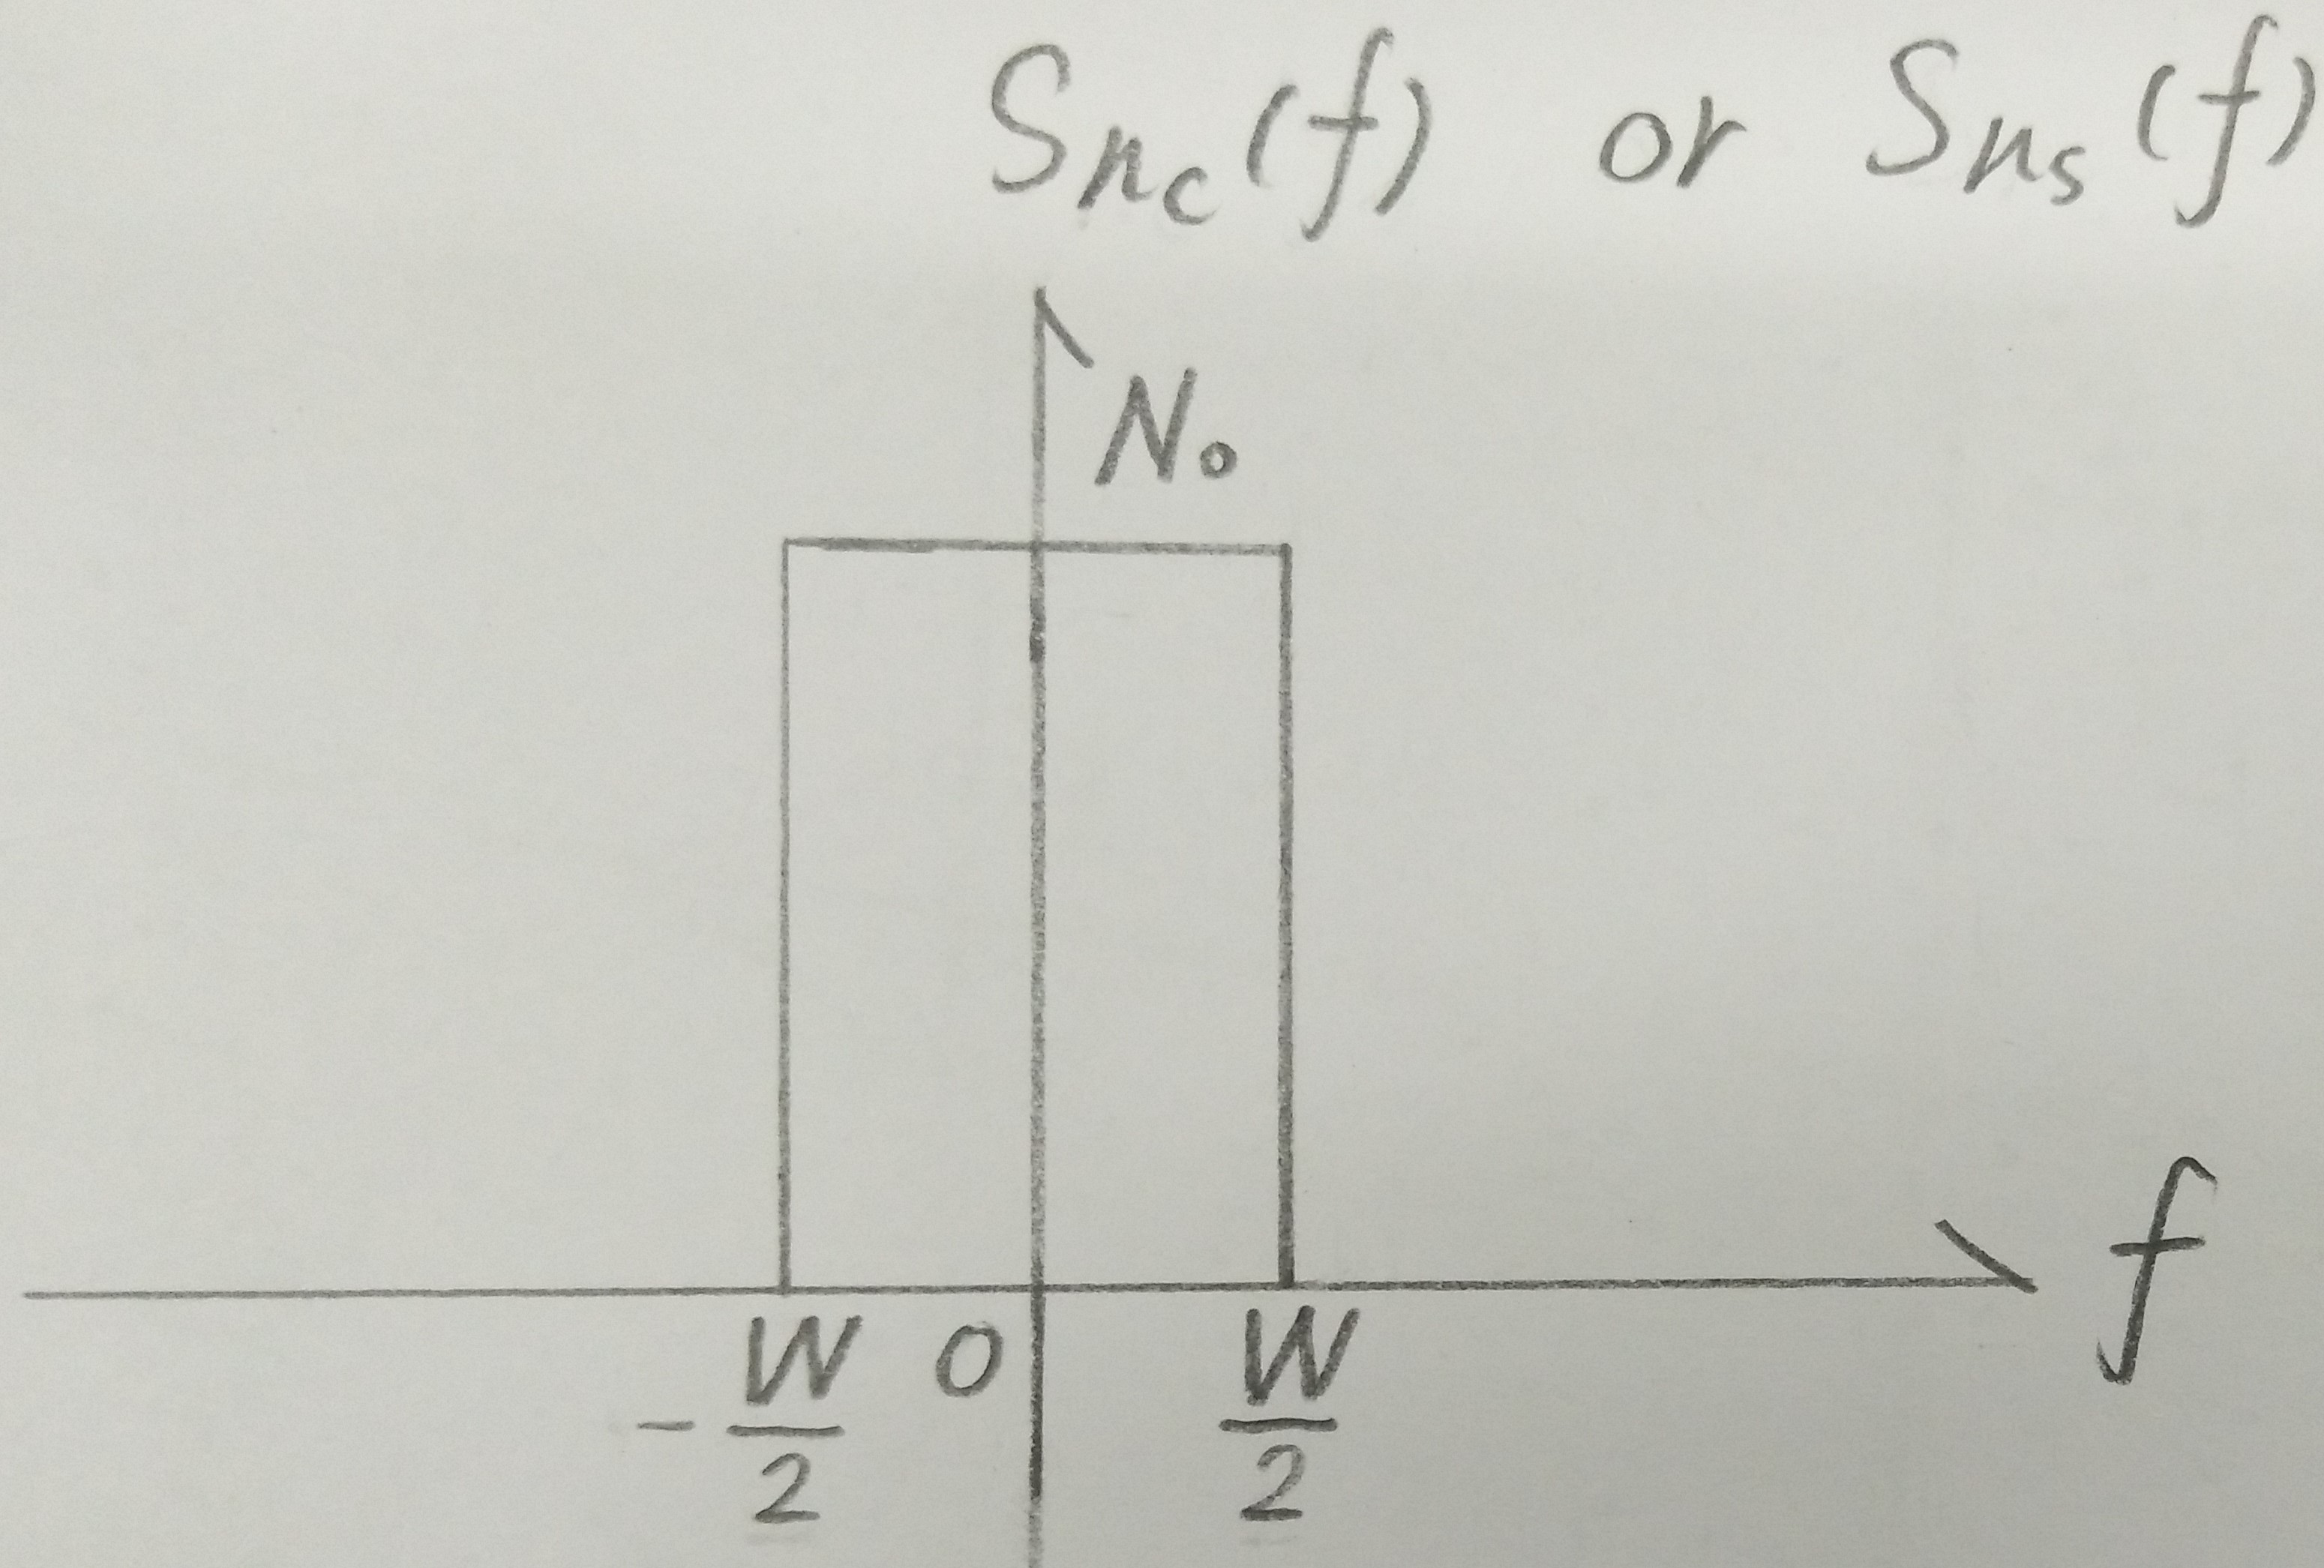
\includegraphics[width=.4\columnwidth]{A-6-P-2.jpg}
        \caption{The power spectral density of the in-phase component $n_c(t)$ and the quadrature component $n_s(t)$}
        \label{P-6-A-2}
    \end{figure}
\end{sol}

\begin{prob}[Noise in AM Receiver, 25pts]
    Assume an AM system operates with a modulation index $a=0.4$. The message signal is $m(t)=5\cos(10\pi t)$.
    \begin{itemize}
        \item[1)] Compute the transmission efficiency.
        \item[2)] Assume the envelope detector operates above the threshold. Compute the output SNR (postdetection SNR) in decibel relative to the input SNR.
        \item[3)] Compute the output SNR in decibels relative to the baseband SNR ($P_T/N_0W$).
        \item[4)] Keep $P_T$ (the average power of modulated signal) unchanged, determine the improvement (in decibels) in the output SNR if the modulation index is increased from $0.4$ to $0.8$. (Hint: Since the input SNR and baseband SNR are unchanged, we can calculate the improvement of output SNR based on its relationship with the input SNR and baseband SNR.)
    \end{itemize}
\end{prob}
\begin{sol}
    \begin{itemize}
        \item[1)] In AM modulation,
        \begin{align}
            m_n(t)=\frac{m(t)}{\abs{\min[m(t)]}}=\cos(10\pi t).
        \end{align}
        The transmission efficiency is
        \begin{align}
            \mu=\frac{a^2\overline{m_n^2(t)}}{a^2\overline{m_n^2(t)}+1}=\frac{a^2/2}{a^2/2+1}=\frac{2}{27}{\color{red}=7.41\%}.
        \end{align}
        \item[2)] The AM modulated signal is
        \begin{align}
            x_c(t)=A_c[1+am_n(t)]\cos(2\pi f_ct+\theta).
        \end{align}
        The received signal is
        \begin{align}
            x_c(t)=x_c(t)+w(t).
        \end{align}
        After passing the bandpass filter, the signal becomes
        \begin{align}
            e_2(t)=A_c[1+am_n(t)]\cos(2\pi f_ct+\theta)+n_c(t)\cos(2\pi f_ct+\theta)-n_s(t)\sin(2\pi f_ct+\theta)=r(t)\cos[2\pi f_ct+\phi(t)],
        \end{align}
        where the envelope of the signal is
        \begin{align}
            r(t)=\sqrt{\{A_c[1+am_n(t)]+n_c(t)\}^2+n_s^2(t)}.
        \end{align}
        The average power of the modulated signal is
        \begin{align}
            P_t=\overline{\{A_c[1+am_n(t)]\cos(2\pi f_ct+\theta)\}^2}=\frac{A_c^2}{2}\left[1+a^2\overline{m_n^{\color{red}2}(t)}\right].
        \end{align}
        The average power of the narrowband noise is $2N_0W$. Therefore, the input SNR is
        \begin{align}
            \text{SNR}_T=\frac{P_T}{2N_0W}=\frac{A_c^2\left[1+a^2\overline{m_n^{\color{red}2}(t)}\right]}{4N_0W}.
        \end{align}
        After the envelope detector, the output signal is the envelope
        \begin{align}
            y_D(t)=r(t)=\sqrt{\{A_c[1+am_n(t)]+n_c(t)\}^2+n_s^2(t)}.
        \end{align}
        Since the envelope detector operates above the threshold, i.e., $\text{SNR}_T$ is large and thus $\abs{A_c[1+am_n(t)]+n_c(t)}\gg\abs{n_s(t)}$,
        \begin{align}
            y_D(t)\approx A_c[1+am_n(t)]+n_c(t).
        \end{align}
        The average of the modulated signal after removal of DC component is
        \begin{align}
            P_D=\overline{[A_cam_n(t)]^2}=A_c^2a^2\overline{m_n^2(t)}.
        \end{align}
        The average power of the noise in the output signal is $2N_0W$. Therefore, the output SNR is
        \begin{align}
            \text{SNR}_D=\frac{P_D}{2N_0W}=\frac{A_c^2a^2\overline{m_n^2(t)}}{2N_0W}.
        \end{align}
        The output SNR in decibels relative to the input SNR is
        \begin{align}
            10\lg\frac{\text{SNR}_D}{\text{SNR}_T}=10\lg\frac{2a^2\overline{m_n^2(t)}}{1+a^2\overline{m_n^2(t)}}=10\lg 2\mu=-8.29(\mathrm{dB}).
        \end{align}
        \item[3)] The average power of the modulated signal is $P_T=\frac{A_c^2}{2}[1+a^2\overline{m_n^2(t)}]$ and the average power of the noise in the message bandwidth is $N_0W$, so the baseband SNR is
        \begin{align}
            \text{SNR}_c=\frac{P_T}{N_0W}=\frac{A_c^2[1+a^2\overline{m_n^2(t)}]}{2N_0W}.
        \end{align}
        The output SNR in decibels relative to the baseband SNR is
        \begin{align}
            10\lg\frac{\text{SNR}_D}{\text{SNR}_c}=10\lg\frac{a^2\overline{m_n^2(t)}}{1+a^2\overline{m_n^2(t)}}=10\lg\mu=-11.30(\mathrm{dB}).
        \end{align}
        \item[4)] Since the baseband SNR is unchanged, we can calculate the improvement of output SNR based on its relation with the baseband SNR:
        \begin{align}
            \notag 10\lg\frac{\text{SNR}_D(a=0.8)}{\text{SNR}_D(a=0.4)}=&10\lg\frac{\text{SNR}_D(a=0.8)/\text{SNR}_c}{\text{SNR}_D(a=0.4)/\text{SNR}_c}=10\lg\frac{\text{SNR}_D(a=0.8)}{\text{SNR}_c}-10\lg\frac{\text{SNR}_D(a=0.4)}{\text{SNR}_c}\\
            =&10\lg\mu(a=0.8)-10\lg(a=0.4)=5.15\mathrm{dB}.
        \end{align}
        The output SNR improves by $5.15$ dB.
    \end{itemize}
\end{sol}

\begin{prob}[Noise in FM Receiver and FDM, 20pts]
    An FDM system uses single-sideband modulation to from the baseband, and FM modulation for transmission of the baseband. Assume that there are eight channels and that all eight message signal have equal power $P_0$ and equal bandwidth $W$. For each signal, only the upper sideband is transmitted. The sub-carrier waves used for the first stage of modulation are defined by $c_k(t)=A_k\cos(2\pi kf_0t),0\leq k\leq 7$. The width of the guardbands is $3W$. The received signal consists of the transmitted FM signal plus white Gaussian noise of zero mean and two-sided power spectral density $N_0/2$. Assume the frequency discriminator at the receiver operates above the threshold.
    \begin{itemize}
        \item[1)] Sketch the power spectral density of the signal produced at the frequency discriminator output, showing both the signal and the noise components.
        \item[2)] Find the relationship between the subcarrier amplitudes $A_k$ such that the SSB modulated signals corresponding to different channels have equal output SNRs at the frequency discriminator output.
    \end{itemize}
\end{prob}
\begin{sol}
    \begin{itemize}
        \item[1)] Since each message signal have equal bandwidth $W$ and the width of the guardbands is $3W$, we have
        \begin{align}
            f_1=\text{\sout{$5$}}{\color{red}4}W,
        \end{align}
        and the $k$th channel occupies the frequency range
        \begin{align}
            \text{\sout{$5kW=kf_1\leq f\leq W+kf_1=(5k+1)W,\quad-(1+5k)W=-W-kf_1\leq f\leq-kf_1=-5kW.$}}
        \end{align}
        \begin{align}
            \color{red}4kW=kf_1\leq f\leq W+kf_1=(4k+1)W,\quad-(1+4k)W=-W-kf_1\leq f\leq-kf_1=-4kW.
        \end{align}
        Since received signal includes the white Gaussian noise of two-sided power spectral density $N_0/2$, the power spectral density of the noise component is
        \begin{align}
            S_n(f)=\frac{K_D^2}{A_c^2}N_0f^2.
        \end{align}
        The power spectral density of the signal and the noise components are shown in figure \ref{A-6-P-4}.
        \begin{figure}[h]
            \centering
            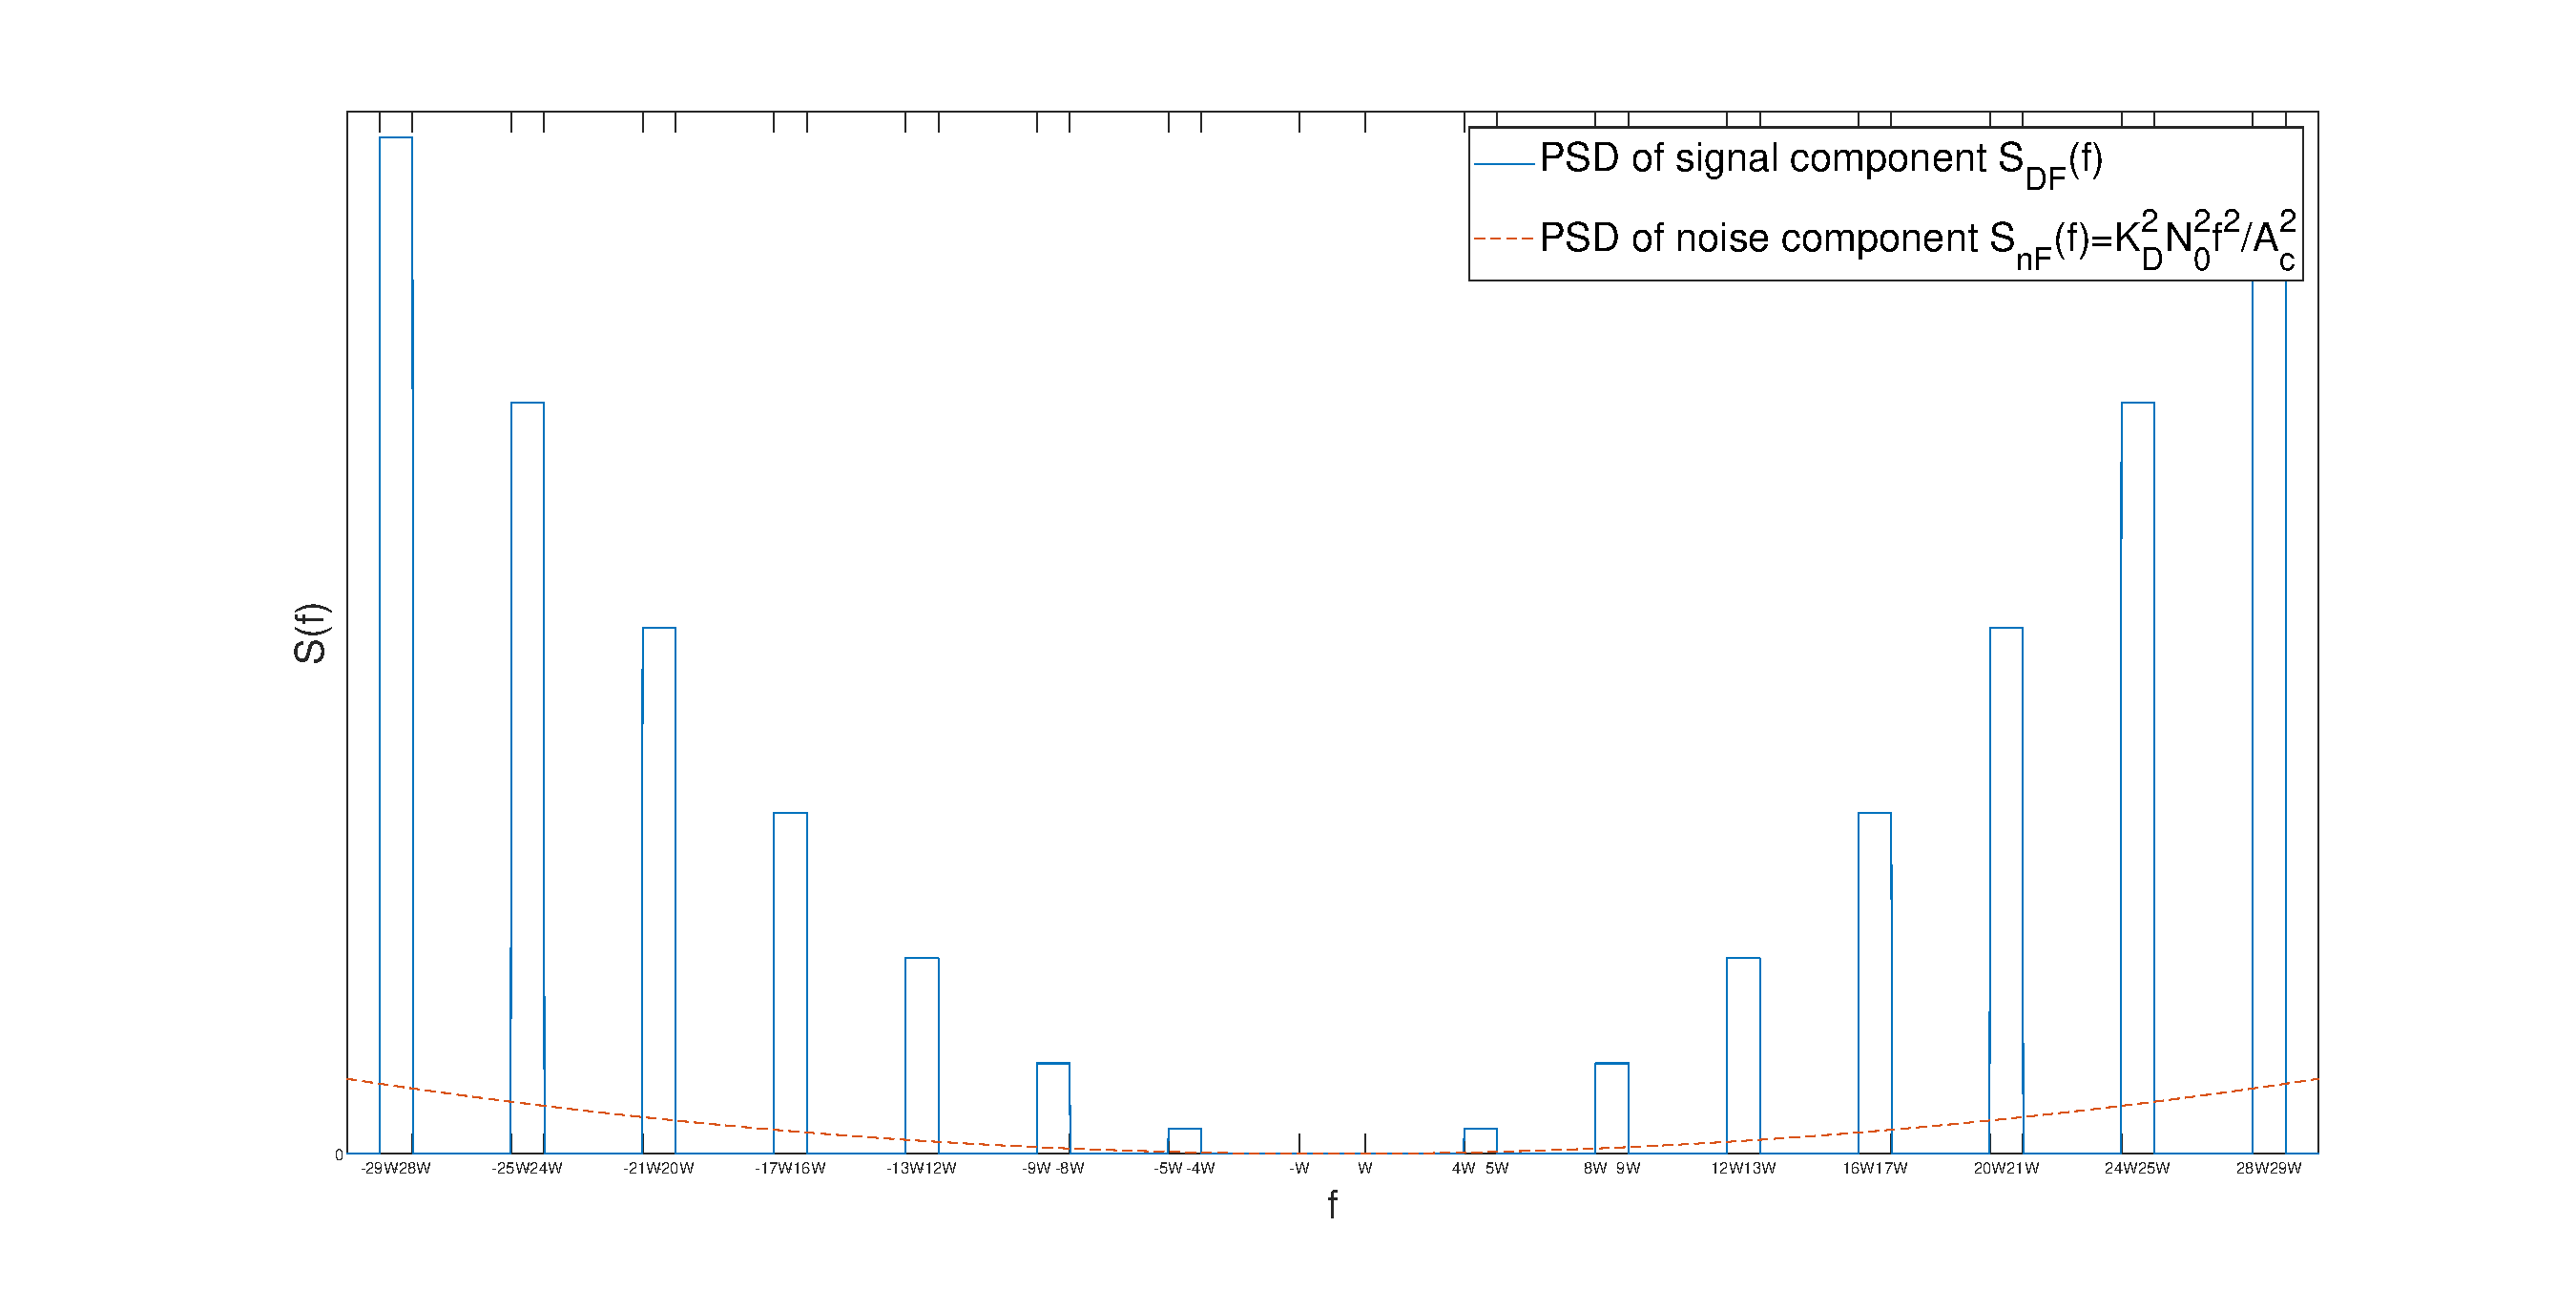
\includegraphics[width=1\columnwidth]{A-6-P-4.eps}
            \caption{The power spectral density of the signal and the noise components}
            \label{A-6-P-4}
        \end{figure}
        \item[2)] The noise power in the $k$th channel is
        \begin{align}
            \text{\sout{$P_{nk}=2\int_{5kW}^{(5k+1)W}S_n(f)\,\mathrm{d}f=2\int_{5kW}^{(5k+1)W}\frac{K_D^2}{A_c^2}N_0f^2\,\mathrm{d}f=\frac{2}{3}\frac{K_D^2}{A_c^2}N_0(75k^2+15k+1)W^3.$}}
        \end{align}
        \begin{align}
            \color{red}P_{nk}=2\int_{4kW}^{(4k+1)W}S_n(f)\,\mathrm{d}f=2\int_{4kW}^{(4k+1)W}\frac{K_D^2}{A_c^2}N_0f^2\,\mathrm{d}f=\frac{2}{3}\frac{K_D^2}{A_c^2}N_0(75k^2+15k+1)W^3.
        \end{align}
        The signal power of each channel is
        \begin{align}
            \text{\sout{$P_T=$}}\left\{\begin{array}{ll}
                \text{\sout{$\frac{K_D^2f_d^2A_k^2}{2},$}}&\text{\sout{$k=0$}}\\
                \text{\sout{$\frac{K_D^2f_d^2A_k^2}{4},$}}&\text{\sout{$1\leq k\leq 7.$}}
            \end{array}\right.{\color{red}P_T=\frac{K_D^2f_d^2A_k^2}{4}.}
        \end{align}
        The output of the $k$th channel is
        \begin{align}
            \text{SNR}_D=\frac{P_T}{P_{nk}}=\left\{\begin{array}{ll}
                \text{\sout{$\frac{3}{4}\frac{f_d^2A_c^2W^3}{N_0}\frac{A_k^2}{75k^2+15k+1}=\frac{3}{4}\frac{f_d^2A_c^2W^3}{N_0}A_0^2,$}}&\text{\sout{$k=0$}},\\
                \text{\sout{$\frac{3}{8}\frac{f_d^2A_c^2W^3}{N_0}\frac{A_k^2}{75k^2+15k+1},$}}&\text{\sout{$1\leq k\leq 7.$}}
            \end{array}\right.{\color{red}\frac{3}{8}\frac{f_d^2A_c^2W^3}{N_0}\frac{A_k^2}{48k^2+12k+1}.}
        \end{align}
        To make that the SSB modulated signals corresponding to different channels have equal output SNRs at the frequency dicriminator output,
        \begin{align}
            2A_0^2=\text{\sout{$\frac{A_k^2}{75k^2+15k+1}$}}{\color{red}\frac{A_k^2}{48k^2+12k+1}}=\text{constant},\quad\forall\text{\sout{$1$}}{\color{red}0}\leq k\leq 7.
        \end{align}
    \end{itemize}
\end{sol}
\end{document}